%%%%%%%%%%%%%%%%%%%%%%%%%%%%%%%%%%%
%This is the LaTeX ARTICLE template for RSC journals
%Copyright The Royal Society of Chemistry 2016
%%%%%%%%%%%%%%%%%%%%%%%%%%%%%%%%%%%

\documentclass[twoside,twocolumn,9pt]{article}
\usepackage{extsizes}
\usepackage[super,sort&compress,comma]{natbib} 
\usepackage[version=3]{mhchem}
\usepackage[left=1.5cm, right=1.5cm, top=1.785cm, bottom=2.0cm]{geometry}
\usepackage{balance}
\usepackage{times,mathptmx}
\usepackage{sectsty}
\usepackage{graphicx} 
\usepackage{lastpage}
\usepackage[format=plain,justification=justified,singlelinecheck=false,font={stretch=1.125,small,sf},labelfont=bf,labelsep=space]{caption}
\usepackage{float}
\usepackage{fancyhdr}
\usepackage{fnpos}
\usepackage[english]{babel}
\usepackage{array}
\usepackage{droidsans}
\usepackage{charter}
\usepackage[T1]{fontenc}
\usepackage[usenames,dvipsnames]{xcolor}
\usepackage{setspace}
\usepackage[compact]{titlesec}
%%%Please don't disable any packages in the preamble, as this may cause the template to display incorrectly.%%%
\usepackage[obeyFinal]{easy-todo}
\usepackage{url}
\usepackage{rotating}


\usepackage{epstopdf}%This line makes .eps figures into .pdf - please comment out if not required.

\definecolor{cream}{RGB}{222,217,201}

\begin{document}

\pagestyle{fancy}
\thispagestyle{plain}
\fancypagestyle{plain}{

%%%HEADER%%%
\fancyhead[C]{
\includegraphics[width=18.5cm]{head_foot/header_bar}}
\fancyhead[L]{\hspace{0cm}\vspace{1.5cm}
\includegraphics[height=30pt]{head_foot/journal_name}}
\fancyhead[R]{\hspace{0cm}\vspace{1.7cm}
\includegraphics[height=55pt]{head_foot/RSC_LOGO_CMYK}}
\renewcommand{\headrulewidth}{0pt}
}
%%%END OF HEADER%%%

%%%PAGE SETUP - Please do not change any commands within this section%%%
\makeFNbottom
\makeatletter
\renewcommand\LARGE{\@setfontsize\LARGE{15pt}{17}}
\renewcommand\Large{\@setfontsize\Large{12pt}{14}}
\renewcommand\large{\@setfontsize\large{10pt}{12}}
\renewcommand\footnotesize{\@setfontsize\footnotesize{7pt}{10}}
\makeatother

\renewcommand{\thefootnote}{\fnsymbol{footnote}}
\renewcommand\footnoterule{\vspace*{1pt}% 
\color{cream}\hrule width 3.5in height 0.4pt \color{black}\vspace*{5pt}} 
\setcounter{secnumdepth}{5}

\makeatletter 
\renewcommand\@biblabel[1]{#1}            
\renewcommand\@makefntext[1]% 
{\noindent\makebox[0pt][r]{\@thefnmark\,}#1}
\makeatother 
\renewcommand{\figurename}{\small{Fig.}~}
\sectionfont{\sffamily\Large}
\subsectionfont{\normalsize}
\subsubsectionfont{\bf}
\setstretch{1.125} %In particular, please do not alter this line.
\setlength{\skip\footins}{0.8cm}
\setlength{\footnotesep}{0.25cm}
\setlength{\jot}{10pt}
\titlespacing*{\section}{0pt}{4pt}{4pt}
\titlespacing*{\subsection}{0pt}{15pt}{1pt}
%%%END OF PAGE SETUP%%%

%%%FOOTER%%%
\fancyfoot{}
\fancyfoot[LO,RE]{\vspace{-7.1pt}
\includegraphics[height=9pt]{head_foot/LF}}
\fancyfoot[CO]{\vspace{-7.1pt}\hspace{13.2cm}
\includegraphics{head_foot/RF}}
\fancyfoot[CE]{\vspace{-7.2pt}\hspace{-14.2cm}
\includegraphics{head_foot/RF}}
\fancyfoot[RO]{\footnotesize{\sffamily{1--\pageref{LastPage} ~\textbar  \hspace{2pt}\thepage}}}
\fancyfoot[LE]{\footnotesize{\sffamily{\thepage~\textbar\hspace{3.45cm} 1--\pageref{LastPage}}}}
\fancyhead{}
\renewcommand{\headrulewidth}{0pt} 
\renewcommand{\footrulewidth}{0pt}
\setlength{\arrayrulewidth}{1pt}
\setlength{\columnsep}{6.5mm}
\setlength\bibsep{1pt}
%%%END OF FOOTER%%%

%%%FIGURE SETUP - please do not change any commands within this section%%%
\makeatletter 
\newlength{\figrulesep} 
\setlength{\figrulesep}{0.5\textfloatsep} 

\newcommand{\topfigrule}{\vspace*{-1pt}% 
\noindent{\color{cream}\rule[-\figrulesep]{\columnwidth}{1.5pt}} }

\newcommand{\botfigrule}{\vspace*{-2pt}% 
\noindent{\color{cream}\rule[\figrulesep]{\columnwidth}{1.5pt}} }

\newcommand{\dblfigrule}{\vspace*{-1pt}% 
\noindent{\color{cream}\rule[-\figrulesep]{\textwidth}{1.5pt}} }

\makeatother
%%%END OF FIGURE SETUP%%%

%%%TITLE, AUTHORS AND ABSTRACT%%%
\twocolumn[
  \begin{@twocolumnfalse}
\vspace{3cm}
\sffamily
\begin{tabular}{m{4.5cm} p{13.5cm} }


\includegraphics{head_foot/DOI} & \noindent\LARGE{\textbf{Molecular electrometer and binding of cations to phospholipid bilayers$^\dag$}} \\%Article title goes here instead of the text "This is the title"
\vspace{0.3cm} & \vspace{0.3cm} \\

 & \noindent\large{Andrea Catte,\textit{$^{a\ddag}$} Mykhailo Girych,\textit{$^{b}$} Matti Javanainen,\textit{$^{c,d}$} Claire Loison,\textit{$^{e}$} Josef Melcr,\textit{$^{f}$} Markus S. Miettinen,\textit{$^{g,h}$} Luca Monticelli,\textit{$^{i}$} Jukka M{\"a}{\"a}tt{\"a},\textit{$^{j}$} Vasily S. Oganesyan,\textit{$^{a}$} O. H. Samuli Ollila,\textit{$^{\ast b}$} Joona Tynkkynen,\textit{$^{c}$} and Sergey Vilov,\textit{$^{e}$}
} \\%Author names go here instead of "Full name", etc.


\includegraphics{head_foot/dates} & \noindent\normalsize{
%The abstract should be a single paragraph which summarises the content of the article. Any references in the abstract should be written out in full \textit{e.g.}\ [Surname \textit{et al., Journal Title}, 2000, \textbf{35}, 3523].
Despite the vast amount of experimental and theoretical studies on the binding affinity of cations into phosholipid bilayers, 
especially the biologically relevant Na$^+$ and Ca$^{2+}$ ions,  there is no consensus in the literature. 
In this paper, we show that the ion binding affinity can be directly compared between simulations and experiments by 
using the choline headgroup order parameters according to the 'molecular electrometer' concept.%~\cite{seelig87}.
Our findings strongly support the pre-2000 view that Na$^+$ and other monovalent ions
(except Li$^+$) do not specifically bind to phosphatidylcholine lipid bilayers with mM concentrations, 
in contrast to Ca$^{2+}$ and other multivalent ions. Especially the Na$^+$ binding affinity is 
overestimated by several molecular dynamics simulation models, leading to 
an artificially positively charged lipid bilayer and overexagerated structural effects in the headgroups. 
Qualitatively correct headgroup order parameter response is observed with
Ca$^{2+}$ binding in all the tested models, however, none of the them has a sufficient 
quantitative accuracy to interpret the Ca$^{2+}$:lipid stoichiometry or the induced atomistic resolution structural changes.
This work has been done as a fully open collaboration, using \url{nmrlipids.blogspot.fi} as a main communication platform; 
all the scientific contributions were made publicly on this blog. } \\%The abstrast goes here instead of the text "The abstract should be..."

\end{tabular}

 \end{@twocolumnfalse} \vspace{0.6cm}

  ]
%%%END OF TITLE, AUTHORS AND ABSTRACT%%%

%%%FONT SETUP - please do not change any commands within this section
\renewcommand*\rmdefault{bch}\normalfont\upshape
\rmfamily
\section*{}
\vspace{-1cm}


%%%FOOTNOTES%%%

\footnotetext{\textit{$^{a}$~University of East Anglia, Norwich, United Kingdom}}
\footnotetext{\textit{$^{b}$~Department of Biomedical Engineering and Computational Science, Aalto University, Espoo, Finland}}
\footnotetext{\textit{$^{c}$~Tampere University of Technology, Tampere, Finland}}
\footnotetext{\textit{$^{d}$~University of Helsinki,Finland}}
\footnotetext{\textit{$^{e}$~Institut Lumi{\'e}re Mati{\'e}re, UMR5306 Universit{\'e} Lyon 1-CNRS, Universit{\'e} de Lyon, 69622 Villeurbanne, France}}
\footnotetext{\textit{$^{f}$~Institute of Organic Chemistry and Biochemistry, Czech Academy of Sciences, Flemingovo n{\'a}m. 2, 16610 Prague 6, Czech Republic, Charles University in Prague, Faculty of Mathematics and Physics, Ke Karlovu 3, 121 16 Prague 2, Czech Republic}}
\footnotetext{\textit{$^{g}$~Fachbereich Physik, Freie Universit\"at Berlin, Berlin, Germany}}
\footnotetext{\textit{$^{h}$~Max Planck Institute of Colloids and Interfaces, Department of Theory and Bio-Systems, Potsdam, Germany}}
\footnotetext{\textit{$^{i}$~Institut de Biologie et Chimie des Prot{\'e}ines (IBCP), CNRS UMR 5086, Lyon, France}}
\footnotetext{\textit{$^{j}$~Aalto University, Espoo, Finland}}
\footnotetext{\textit{$^{\ast}${\bf Author to whom correspondence may be addressed. E-mail: samuli.ollila@aalto.fi.}}}


%\footnotetext{\textit{$^{b}$~Address, Address, Town, Country. Fax: XX XXXX XXXX; Tel: XX XXXX XXXX; E-mail: xxxx@aaa.bbb.ccc}} }}



%Please use \dag to cite the ESI in the main text of the article.
%If you article does not have ESI please remove the the \dag symbol from the title and the footnotetext below.
\footnotetext{\dag~Electronic Supplementary Information (ESI) available: %[details of any supplementary information available should be included here]. 
5 figures, detailed technical discussion and simulation details.
See DOI: 10.1039/b000000x/}
%additional addresses can be cited as above using the lower-case letters, c, d, e... If all authors are from the same address, no letter is required

\footnotetext{\ddag~The authors are listed in alphaphetical order. 
%Additional footnotes to the title and authors can be included \textit{e.g.}\ `Present address:' 
%or `These authors contributed equally to this work' as above using the symbols: \ddag, \textsection, 
%and \P. Please place the appropriate symbol next to the author's name and include a \texttt{\textbackslash footnotetext} 
%entry in the the correct place in the list.
}


%%%END OF FOOTNOTES%%%

%%%MAIN TEXT%%%%


\section{Introduction}

Due to its high physiological importance --- nerve cell signalling being the prime example ---
interaction of cations with phospholipid membranes
has been widely studied via theory, simulations, and experiments.
The relative ion binding affinities are generally agreed to
follow the Hofmeister series~\cite{eisenberg79,cevc90,tocanne90,binder02,celma07,leontidis09,vacha09a,klasczyk10,harb13}, 
however,
consensus on the quantitative affinities is currently lacking.
Until 1990, the consensus (documented in two extensive reviews~\cite{cevc90,tocanne90}) was that
while  multivalent cations interact significantly with phospholipid bilayers,
for monovalent cations (with the exception of Li$^+$) the interactions are weak.
This conclusion has since been strengthened by further
studies showing that bilayer properties remain unaltered upon the addition of sub-molar concentrations of monovalent 
salt~\cite{binder02,pabst07,filippov09}.
Since 2000, however, another view has emerged, suggesting much stronger interactions between phospholipids and monovalent cations, and strong Na$^{+}$ binding in particular~\cite{bockmann03,bockmann04,vacha09a,manyes05,manyes06,fukuma07,leontidis09,ferber11,morata12,klasczyk10,harb13}.

The pre-2000 view has the experimental support that
(in contrast to the significant effects caused by any multivalent cations)
sub-molar concentrations of NaCl have a negligible effect on
phospholipid infrared spectra~\cite{binder02},
area per molecule~\cite{pabst07},
dipole potential~\cite{clarke99},
lateral diffusion~\cite{filippov09},
and choline head group order parameters~\cite{akutsu81};
in addition, the water sorption isotherm of a NaCl--phospholipid system
is highly similar to that of a  pure NaCl solution
--- indicating that the ion--lipid interaction is very weak~\cite{binder02}. 

The post-2000 'strong binding' view rests on experimental and above all simulational findings.
At sub-molar NaCl concentrations, the rotational and translational dynamics of membrane-embedded fluorescent probes decrease~\cite{bockmann03,vacha09a,harb13}, and Atomic Force Microscopy (AFM) experiments show changes in bilayer hardness~\cite{manyes05,manyes06,fukuma07,ferber11,morata12};
in atomistic molecular dynamics (MD) simulations, phospholipid bilayers consistently bind Na${^+}$,
although the binding strength depends on the model used~\cite{bockmann03,bockmann04,sachs04,berkowitz06,cordomi08,cordomi09,valley11,berkowitz12}.

Some observables have been interpreted in favor of both views. For example,
as the effect of monovalent ions (except Li$^+$)  on the phase transition temperature is tiny
(compared to the effect of multivalent ions), it was initially interpreted 
as an indication that only multivalent ions and Li$^+$ specifically bind to phosholipid bilayers~\cite{cevc90}; 
however, such a small effect in calorimetric measurements was later interpreted to indicate that also
Na$^+$ binds~\cite{bockmann03,klasczyk10}.
Similarly, the lack of significant positive electrophoretic mobility
of phosphatidylcholine (PC) vesicles in the presence of NaCl
(again in contrast to multivalent ions and Li$^+$)
suggested weak binding of Na$^+$~\cite{eisenberg79,tatulian87,manyes05,manyes06,klasczyk10};
%NaCl increases the (initially negative) zeta potential to only about zero,
%whereas positive zeta potentials are generally reached with
however, these data have also been explained by a countering effect of the Cl$^-$ ions~\cite{berkowitz06,knecht13}.
To reduce the area per lipid in scattering experiments, molar concentrations of NaCl are required~\cite{pabst07}, which indicates weak ion--lipid interaction;
in MD simulations, however, already orders of magnitude lower concentrations result in Na$^+$ binding and clear reduction of area per lipid.
Finally,  in noninvasive NMR experiments, lipid lateral diffusion is unaltered by NaCl~\cite{filippov09};
%suggesting that the fluorescence results arise from Na$^{+}$ interactions with probes rather than with lipids.
%This is pointed out in Conclusions, which I think is the best place for it. -markus.
however, it is reduced in simulations upon Na$^+$ binding,
which supports interpreting the reduced lateral diffusion of fluorescent probes~\cite{bockmann03,vacha09a,harb13}
as favoring the post-2000 view.

In this paper we set out to solve the apparent contradictions
between the pre-2000 and post-2000 views.
To this end we employ the 'molecular electrometer' concept,
according to which the changes in the order parameters of the $\alpha$ and $\beta$ carbons 
in the phospholipid head group (see Fig. \ref{POPCstructure}) can be used to measure the ion affinity to 
PC lipid bilayer~\cite{akutsu81,altenbach84,seelig87,scherer89}.
As order parameters can be accurately measured in experiments and directly compared to 
simulations \cite{ollila16}, employing the molecular electrometer as a function of cation concentration allows the 
comparison of binding affinity between simulations and experiments.
In addition to demonstrating the usefulness of this general concept,
we show that the response of order parameters to penetrating cations
is qualitatively correct in MD simulations, but that in several  models the affinity of Na$^{+}$ for PC bilayers
is grossly overestimated.
Moreover, we show that the accuracy of lipid--Ca$^{2+}$ interactions 
in current models is not enough for atomistic resolution interpretation of NMR experiments. 

This work has been done as an Open Collaboration at \url{nmrlipids.blogspot.fi};
all the related files (\url{https://github.com/NMRLipids/lipid_ionINTERACTION})
and almost all the simulation data (\url{https://zenodo.org/collection/user-nmrlipids})
are openly available.

\begin{figure}[]
  \centering
  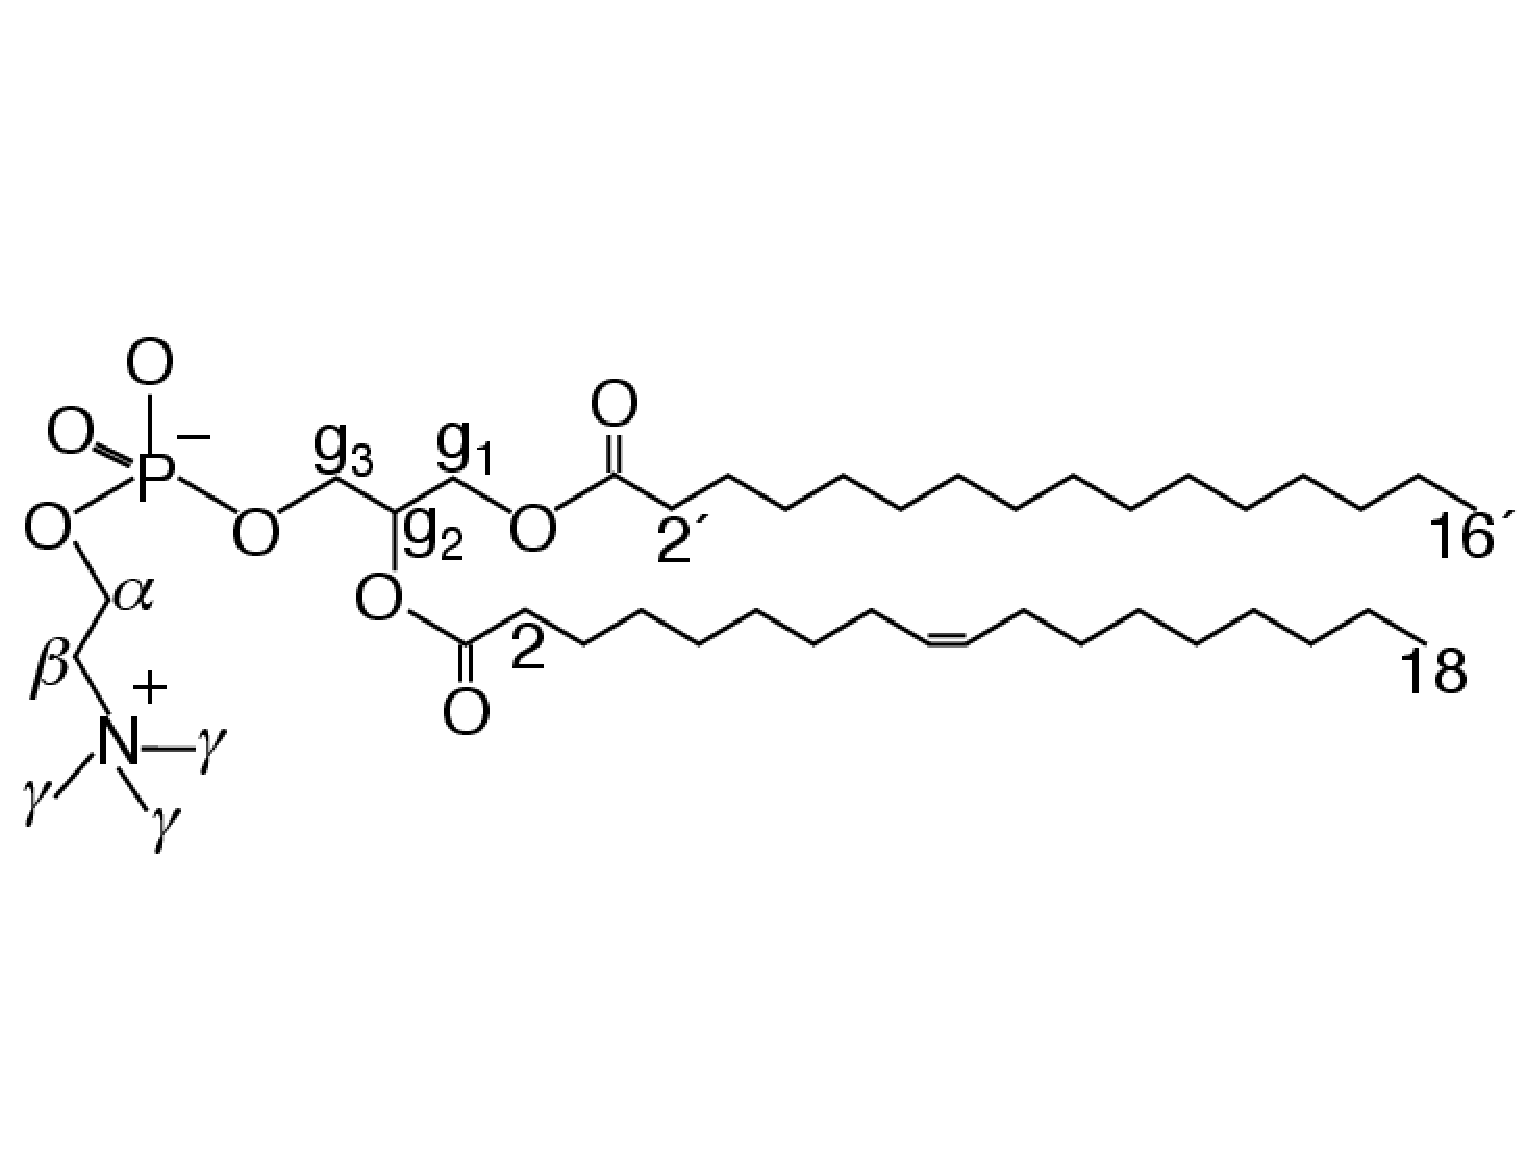
\includegraphics[width=8.6cm]{../Fig/POPCstructure.eps}

  \caption{\label{POPCstructure}
    Chemical structure of 1-palmitoyl-2-oleoylphosphatidylcholine (POPC), and the definition of $\gamma$, $\beta$, $\alpha$, $g_1$, $g_2$ and $g_3$ segments.}
  
\end{figure}


\section{Results and Discussion}

\subsection{Background: Molecular electrometer in experiments}\label{conceptinexperiments}
The molecular electrometer concept is based on the experimental observation that
binding of any charged objects on a PC bilayer interface induces systematic changes in the choline $\beta$ and $\alpha$
segment order parameters~\cite{akutsu81,altenbach84,altenbach85,seelig87,macdonald87,scherer89,roux90,beschiasvili91,marassi92,rydall92}.
Thus, these changes can be used to determine binding affinities of the charged objects.
Molecular electrometer was originally devised for cations~\cite{akutsu81,altenbach84}, but
further experimental quantification with various positively and negatively charged 
molecules showed that the choline order parameters $S_\mathrm{CH}^\alpha$ and $S_\mathrm{CH}^\beta$ 
in general vary linearly with small amount of bound charge per 
lipid~\cite{altenbach84,altenbach85,seelig87,macdonald87,scherer89,roux90,beschiasvili91,marassi92,rydall92}. 
The empirically observed linear relation can be written as~\cite{ferreira16}
\begin{equation}\label{electrometer_eq}
S_{\rm{CH}}^{i}(X^\pm)=S_{\rm{CH}}^{i}(0) + \frac{4m_i}{3\chi} X^\pm,
\end{equation}
where $S_{\rm{CH}}^{i}(0)$ is the order parameter in the absence of bound charges,
$m_i$ empirical constant depending on the valency and position of bound charge,
the quadrupole coupling constant $\chi \approx$ 167 kHz, $X^\pm$ is the amount of bound charge per lipid, and
$i$ refers to either $\alpha$ or $\beta$.
The order parameter change with respect to a bilayer without bound charges then becomes
\begin{equation}\label{OPchangeEQ}
\Delta S_{\rm{CH}}^{i}= S_{\rm{CH}}^{i}(X^\pm)-S_{\rm{CH}}^{i}(0) =\frac{4m_i }{3\chi}X^\pm.
\end{equation}
For Ca$^{2+}$ binding to POPC bilayer (in the presence of 100~mM NaCl),
combination of atomic absorption spectra and $^2$H NMR experiments gave
$m_\alpha=-20.5$  and $m_\beta=-10.0$~\cite{altenbach84}.

\begin{figure*}[t]
  \centering
  \includegraphics[width=15cm]{../Fig/OrderParameterIONSchanges.eps}
  \caption{\label{ordPions}
    The order parameter changes for $\beta$ and $\alpha$ segments as a function of NaCl (left column) 
    and CaCl$_2$ (right column) concentration, from simulations and experiments~\cite{akutsu81} 
    (POPC with CaCl$_2$ from \cite{altenbach84}). The signs of the experimental order parameters, taken from
    experiments without ions~\cite{hong95a,hong95b,gross97}, can be assumed to be unchanged 
    with concentrations represented here~\cite{altenbach84,ollila16}. 
    It should be noted that none of the models used here reproduces the order parameters
    within experimental error for pure PC bilayer without ions, indicating structural inaccuracies with varying severity in all
    models \cite{botan15}. Note that the relatively large decrease in CHARMM36 with 450~mM CaCl$_2$ arise from more equilibrated binding 
    affinity due to long simulation times, see ESI$^\dag$.
  }
\end{figure*}

The absolute values of order parameters 
increase for $\beta$ and decrease for $\alpha$ segment with bound positive charge
and {\it vice versa} for negative charge~\cite{akutsu81,altenbach84,altenbach85,seelig87,scherer89,rydall92}. 
However, as the $\beta$ carbon order parameter is negative while $\alpha$ carbon order parameter is 
positive~\cite{hong95a,hong95b,gross97}, we can conclude 
that both $\Delta S_{\rm{CH}}^{\beta}$ and $\Delta S_{\rm{CH}}^{\alpha}$ decrease with bound positive charge 
and increase with bound negative charge. Consequently, values of $m_i$ are negative for
bound positive charges and {\it vice versa}. This can be rationalized by electrostatically 
induced changes in choline P-N dipole tilt \cite{seelig87,scherer89,seelig90}, which is also
seen in simulations~\cite{gurtovenko05,cordomi08,cordomi09,zhao12}. 
This is in line with order parameter decrease related to the P-N vector tilting more parallel to membrane plane seen with decreasing hydration levels~\cite{botan15}. 


The quantification of $\Delta S_\mathrm{CH}^\beta$ and $\Delta S_\mathrm{CH}^\alpha$
with different cations
have revealed that $\Delta S_{\rm{CH}}^{\beta}/\Delta S_{\rm{CH}}^{\alpha} \approx$0.5 for a wide range
of different cations (aqueous cations, cationic peptides, cationic anesthetics)~\cite{beschiasvili91,rydall92}.
More specifically,
the relation $\Delta S_{\rm{CH}}^{\beta}=0.43 \Delta S_{\rm{CH}}^{\alpha}$ was found for a DPPC bilayer
with various CaCl$_2$ concentrations~\cite{akutsu81}.


\subsection{Molecular electrometer concept in MD simulations}\label{electrometerinsimulations}

The headgroup order parameter changes as a function of ion concentration in
solution from H$^2$ NMR experiments are shown in Fig.~\ref{ordPions} for DPPC and POPC bilayers~\cite{akutsu81,altenbach84}.
Only minor changes in order parameters are seen
as a function of NaCl in solution, 
while the effect of CaCl$_2$ is an order of magnitude larger. 
Thus, according to the molecular electrometer concept, 
monovalent Na$^+$ ions have negligible affinity for PC lipid bilayers at concentrations up to 1 M,
while binding of Ca$^{2+}$ ions at the same concentration is significant~\cite{akutsu81,altenbach84}. 
%({\it Note that in contrast to the response as a function of bound charge in 
%Eq.~\eqref{electrometer_eq}, the changes in Fig.~\ref{ordPions}
%are not linear. This can be explained by electrostatic repulsion between
%already bound calcium ions and ions in solution \cite{altenbach84}.}
%\todo{Is this really needed? The x-axis of Fig.~\ref{ordPions} is not $X^\pm$, so
%why would one even expect the curves to follow Eq.~\eqref{electrometer_eq}?})
%SAMULI: I have removed this now.


Figure~\ref{ordPions} also reports order parameter changes calculated from MD simulations
of DPPC and POPC lipid bilayers as a function of NaCl or CaCl$_2$ concentrations in solution
(for details of the simulated systems see Tables~\ref{IONsystems},~\ref{IONsystems2} and ESI$^\dag$).
Note that none of these MD models
reproduced within experimental uncertainty the order parameters for a pure PC bilayer without ions
(Figure 2 in Ref.~\citenum{botan15}),
indicating structural inaccuracies of varying severity in all models \cite{botan15}.
However, the experimentally observed headgroup order parameter increase with dehydration
was qualitatively reproduced by all the models \cite{botan15}, and 
similarly here the presence of cations leads to the decrease 
of $S_\mathrm{CH}^\beta$ and $S_\mathrm{CH}^\alpha$ (Fig. \ref{ordPions}), in qualitative
agreement with experiments. The changes are, however, overestimated by most models.
According to the electrometer concept this indicates overbinding of cations in most MD simulation
models.

While electrometer concept is well established in experiments (see previous section),
it is not {\it a priori} clear that it works in simulations. The overestimated order parameter
decrease could, in principle, arise also from oversentitivity of choline headgroups on cation binding,
instead of overbinding. Here we analyze the relation between cation binding and choline order 
parameter decrease in simulations in order to evaluate usability of electrometer concept in MD simulations.

According to the molecular electrometer concept, order parameter changes are linearly proportional to
the amount of bound cations in bilayer (Eq.~\eqref{OPchangeEQ}).
Figure~\ref{electrometer} shows the order parameter changes as a function of bound charge in MD simulations;
in keeping with the molecular electrometer, roughly linear correlation between bound charge and order parameter change is found in all models.
Note that quantitative comparison of the proportionality constants (i.e. slopes in Fig. \ref{electrometer})
between different models and experimental slopes
($m_\alpha=-20.5$ and $m_\beta=-10.0$ for Ca$^{2+}$ binding in DPPC bilayer in
the presence of 100mM NaCl in Eq. \ref{electrometer_eq}~\cite{altenbach84}) is not straightforward 
since the simulation slopes depend on the definition used for bound ions. 
\begin{figure}[t]
  \centering
  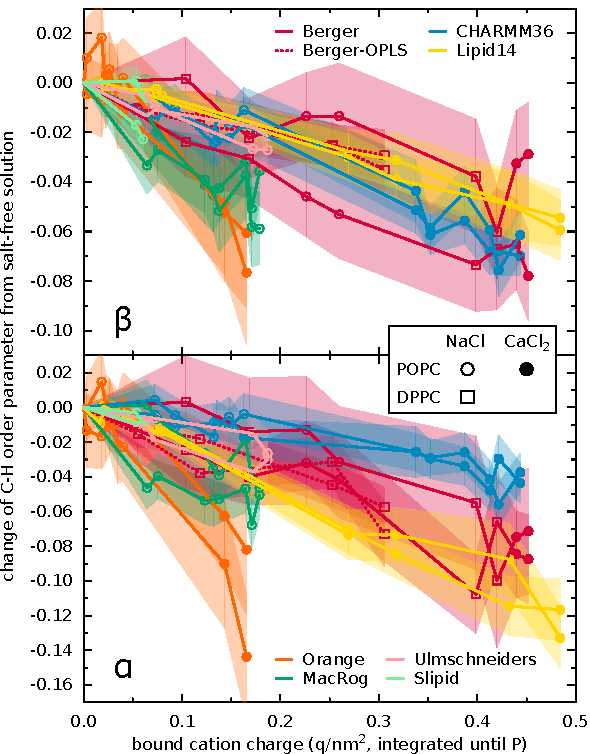
\includegraphics[width=8.6cm]{../scratch/boundIons/dOP_vs_boundCationCharge_P.pdf}
  \caption{\label{electrometer}
    Order parameters changes $\Delta S_{\rm{CH}}^{\beta}$ and $\Delta S_{\rm{CH}}^{\alpha}$ as a function of bound
    cations from different simulation models.
   }
\todo{Results from long CHARMM and Slipids simulations to be added. Description of the calculation of bound charges to be described, probably in supplementary.}
\end{figure}

The comparison of order parameter changes in response to bound charge is more straightforward for
systems with charged amphiphiles fully associated in bilayer, as the amount of bound charge
is then explicitly known in both simulations and experiments. Such comparison
between previously published simulation data \cite{miettinen09} and experiments \cite{scherer89,franzin98}
could not rule out
overestimation of order parameter response to bound cations (i.e., slopes $m_\beta$ and $m_\alpha$)
in a Berger-based model (ESI$^\dag$).
This might, in principle, explain the overestimated order parameter 
response of Berger model to CaCl$_2$, but not to NaCl (see discussion in ESI$^\dag$).
Since simulation data with charged amphiphiles from other models is not available,
the extended comparison with different models is left for further studies.

Figure~\ref{electrometer} shows that the order parameter decrease clearly correlates with the
amount of bound cations also in simulations. This is also evident from Fig.~\ref{NAdensities},
which shows the Na$^+$ density profiles of the MD models
ordered according to the order parameter change 
(reported in Fig.~\ref{ordPions}) from the smallest (top) to the largest (bottom).
The Na$^+$ density peaks are larger for models with larger changes in order parameters,
in line with the observed correlation between cation binding and order parameter decrease in
Fig.~\ref{electrometer}.
\begin{figure}[t]
  \centering
  \includegraphics[width=8cm]{../Fig/NAdensities.eps}
  \caption{\label{NAdensities}
    Atom number density profiles along the membrane normal for lipids, Na$^+$, and Cl$^-$ ions 
    from simulations with different force fields and different NaCl concentrations. 
    The force fields are ordered according to the order parameter changes 
    reported Fig.~\ref{ordPions}, from the smallest (top panel) to the larges (bottom panel).
    The lipid densities are scaled by 100 (united atom) or 200 (all atom model) to improve readability. 
%    Figure discussed in https://github.com/NMRLipids/lipid\_ionINTERACTION/issues/4.
}
\end{figure}

Figure~\ref{AvsB} compares the relation between $\Delta S_{\rm{CH}}^{\beta}$ and $\Delta S_{\rm{CH}}^{\alpha}$
in experiments~\cite{akutsu81} and different simulation models.
Only Lipid14 gives $\Delta S_{\rm{CH}}^{\beta}/\Delta S_{\rm{CH}}^{\alpha}$ ratio in agreement with the experimental ratio.
In all the other models the $\alpha$ order parameter decrease with bound cations is underestimated in
respect to $\beta$ order parameter decrease.
\begin{figure}[t]
  \centering
  \includegraphics[width=8cm]{../Fig/OrderParameterAvsB.eps}
  \caption{\label{AvsB}
    Relation between $\Delta S_{\rm{CH}}^{\beta}$ and $\Delta S_{\rm{CH}}^{\alpha}$ from experiments~\cite{akutsu81} and
    different simulation models. Solid line is $\Delta S_{\rm{CH}}^{\beta}=0.43\Delta S_{\rm{CH}}^{\alpha}$ determined for DPPC bilayer
    from $^2$H NMR experiment with various CaCl$_2$ concentrations~\cite{akutsu81}.
  }
\end{figure}




In conclusion, the clear correlation between bound cations and order parameter decrease 
is observed in all the tested simulation models. Consequently, the electrometer concept can 
be used to compare the cation binding affinity between experiments and simulations. 
However, we find that the quantitative response of $\alpha$ and $\beta$ segment order parameters to bound cations in simulations 
do not generally agree with the experiments. The $\Delta S_{\rm{CH}}^{\beta}/\Delta S_{\rm{CH}}^{\alpha}$ ratio  
agrees with experiments only in Lipid14 model (Fig.~\ref{AvsB}). 
Thus, the observed overestimations of the order parameter changes with cation concentrations may, in principle, arise
from overbinding of ions or from too sensitive lipid headgroup response on bound cation 
(see also discussion in ESI$^\dag$). 
A careful analysis with current lipid models is performed in the next section.

\begin{sidewaystable*}[!p]
\centering
\caption{List of simulations performed in this work. The ion concentrations are calculated as 
   [ion]=(N$_{\rm ion} \times$[water])/N$_{\rm w}$, where [water]=55.5M. 
   These correspond the concentrations reported in the experiments by Akutsu et al.~\cite{akutsu81}.
   The lipid force fields are named as in our previous work~\cite{botan15}.}\label{IONsystems}
\begin{tabular}{c c c c c c c c c c c c}
  %\hline
  % some footnotes are not visible in typeset-MS (pdf)
  Force field (lipid, ion)& lipid & [Ion] mM & \footnote{The number of lipid molecules}N$_{\rm l}$   &  \footnote{The number of water molecules}N$_{\rm w}$   & \footnote{The number of Na$^+$ molecules}N$_{\rm Na}$  & \footnote{The number of Ca$^{2+}$ molecules}N$_{\rm Ca}$   &  \footnote{The number of Cl molecules}N$_{\rm Cl}$ & \footnote{Simulation temperature}T (K)  & \footnote{The total simulation time}t$_{{\rm sim}}$(ns) & \footnote{Time frames used in the analysis}t$_{{\rm anal}}$ (ns) & Files\\
  \hline
  Berger-POPC-07\cite{ollila07a}   &   POPC & 0          & 128 & 7290 & 0  & 0  & 0 & 298  & 270 & 240 & \cite{bergerFILESpopc}  \\
  Berger-POPC-07\cite{ollila07a}, ffgmx\cite{straatsma88}  &   POPC & 340 (NaCl) & 128 & 7202 & 44  & 0  & 44 &298  & 110 & 50 & \cite{bergerPOPC340mMNaClfiles} \\
  %\hdashline
  Berger-POPC-07\cite{ollila07a}, ffgmx\cite{straatsma88}  &   POPC & 340 (CaCl$_2$) & 128 & 7157 & 0 & 44  & 88 &298 & 108 & 58 &\cite{bergerPOPC340mMCaClfiles}  \\
  \hline
  Berger-DPPC-97\cite{marrink98}   &   DPPC & 0 & 72 & 2880 & 0  & 0  & 0 &323  & 60 & 50 &\cite{bergerDPPCfiles} \\
  Berger-DPPC-97\cite{marrink98}, ffgmx\cite{straatsma88}   &   DPPC & 150 (NaCl) & 72 & 2880 & 8  & 0  & 8 &323  & 120 & 60 &\cite{bergerDPPC150mMfiles} \\
  Berger-DPPC-97\cite{marrink98}, ffgmx\cite{straatsma88}   &   DPPC & 1000 (NaCl) & 72 & 2778 & 51  & 0  & 51 &323  & 120 & 60 &\cite{bergerDPPC1000mMfiles} \\
  \hline
  BergerOPLS-DPPC-06\cite{tieleman06} &   DPPC & 0 & 72 & 2880 & 0  & 0  & 0 &323  & 120 & 60 &\cite{bergerOPLSDPPCfiles} \\
  BergerOPLS-DPPC-06\cite{tieleman06}, OPLS\cite{aqvist90} &   DPPC & 150 (NaCl) & 72 & 2880 & 8  & 0  & 8 &323  & 120 & 60 &\cite{bergerOPLSDPPCfiles150mMnacl} \\
  BergerOPLS-DPPC-06\cite{tieleman06}, OPLS\cite{aqvist90} &   DPPC & 1000 (NaCl) & 72 & 2778 & 51  & 0  & 51 &323  & 120 & 60 &\cite{bergerOPLSDPPCfiles1000mMnacl} \\
  \hline
  CHARMM36\cite{klauda10}   & POPC & 0           & 72 & 2242 & 0  & 0 & 0 & 303  & 30 & 20 & \cite{charmm36filesSHORT} \\
  CHARMM36\cite{klauda10}, CHARMM36\cite{venable13} & POPC & 350 (NaCl)  & 72 & 2085 & 13  & 0 & 13 & 303  & 80 & 60 & \cite{charmmPOPC350mMNaClfiles} \\
  CHARMM36\cite{klauda10}, CHARMM36\cite{venable13} & POPC & 690 (NaCl)  & 72 & 2085 & 26  & 0 & 26 & 303  & 73 & 60 & \cite{charmmPOPC690mMNaClfiles}   \\
  CHARMM36\cite{klauda10}, CHARMM36\cite{venable13}  & POPC & 950 (NaCl)  & 72 & 2168 & 37  & 0 & 37 & 303  & 80 & 60 &\cite{charmmPOPC950mMNaClfiles}  \\
  CHARMM36\cite{klauda10}, CHARMM36 & POPC &  350 (CaCl$_2$)  & 128 & 6400 & 0& 35 & 70 & 303  & 200  & 100 & \cite{charmmPOPC350mMCaClfiles}  \\
  CHARMM36\cite{klauda10}, CHARMM36 & POPC &  450 (CaCl$_2$)  & 200 & 9000 & 0& 73 & 146 & 310  & 2000  & 100 & \cite{charmmPOPC450mMCaClfiles}  \\
  CHARMM36\cite{klauda10}, CHARMM36 & POPC &  670 (CaCl$_2$)  & 128 & 6400 & 0& 67 & 134 & 303  & 200  & 120 & \cite{charmmPOPC670mMCaClfiles}  \\  
  CHARMM36\cite{klauda10}, CHARMM36 & POPC &  1000 (CaCl$_2$) & 128 & 6400 & 0& 100 & 200 & 303 & 200  & 100 & \cite{charmmPOPC1000mMCaClfiles}  \\
  \hline
  CHARMM36\cite{klauda10}, Yoo\cite{yoo16}  & DPPC & 430 (CaCl$_2$)  & 128 & 7760 & 60  & 0 & 120 & 323  & 200 & 170 &todo  \\
  CHARMM36\cite{klauda10}, Yoo\cite{yoo16}  & DPPC & 886 (CaCl$_2$)  & 128 & 7520 & 120  & 0 & 240 & 323  & 200 & 170 &todo  \\
  \hline
  MacRog\cite{maciejewski14}  & POPC & 0 & 288 & 14400 & 0 & 0 & 0 & 310 & 90&40  &~\cite{macrogdehydFILES}  \\
  MacRog\cite{maciejewski14}, OPLS\cite{aqvist90}  & POPC & 100 (NaCl) & 288 & 14554 & 27 & 0 & 27 & 310 & 90&50  & \cite{macrogIONfiles} \\
  MacRog\cite{maciejewski14}, OPLS\cite{aqvist90}  & POPC &  210 (NaCl) & 288 & 14500 & 54 & 0 & 54 & 310 & 90&50  &\cite{macrogIONfiles}  \\
  MacRog\cite{maciejewski14}, OPLS\cite{aqvist90}  & POPC &   310 (NaCl) & 288 & 14446 & 81 & 0 & 81 & 310 & 90&50  & \cite{macrogIONfiles} \\
  MacRog\cite{maciejewski14}, OPLS\cite{aqvist90}  & POPC &   420 (NaCl) & 288 & 14392 & 108 & 0 & 108 & 310 & 90& 50  & \cite{macrogIONfiles}  \\
\end{tabular}
\end{sidewaystable*} 

\begin{sidewaystable*}[!p]
\centering
\caption{List of simulations performed in this work. The ion concentrations are calculated as 
   [ion]=(N$_{\rm ion} \times$[water])/N$_{\rm w}$, where [water]=55.5M. 
   These correspond the concentrations reported in the experiments by Akutsu et al.~\cite{akutsu81}.
   The lipid force fields are named as in our previous work~\cite{botan15}.}\label{IONsystems2}
\begin{tabular}{c c c c c c c c c c c c}
  %\hline
  % some footnotes are not visible in typeset-MS (pdf)
  Force field (lipid, ion)& lipid & [Ion] mM & \footnote{The number of lipid molecules}N$_{\rm l}$   &  \footnote{The number of water molecules}N$_{\rm w}$   & \footnote{The number of Na$^+$ molecules}N$_{\rm Na}$  & \footnote{The number of Ca$^{2+}$ molecules}N$_{\rm Ca}$   &  \footnote{The number of Cl molecules}N$_{\rm Cl}$ & \footnote{Simulation temperature}T (K)  & \footnote{The total simulation time}t$_{{\rm sim}}$(ns) & \footnote{Time frames used in the analysis}t$_{{\rm anal}}$ (ns) & Files\\
  \hline
  Orange, OPLS\cite{aqvist90}  &   POPC & 0 & 72 & 2880 & 0 & 0  & 0 & 298 & 60 & 50 & \cite{orangePOPCfiles}  \\
  Orange, OPLS\cite{aqvist90} &   POPC & 140 (NaCl) & 72 & 2866 & 7 & 0  & 7 & 298 & 120 & 60 &\cite{orangePOPC140mMNaClfiles}  \\
  Orange, OPLS\cite{aqvist90}  &   POPC & 510 (NaCl) & 72 & 2802 & 26 & 0  & 26 & 298 & 120 & 100 &\cite{orangePOPC510mMNaClfiles}   \\
  Orange, OPLS\cite{aqvist90}  &   POPC & 1000 (NaCl) & 72 & 2780 & 50 & 0  & 50 & 298 & 120 & 80 & \cite{orangePOPC1000mMNaClfiles} \\
  %\hdashline
  Orange, OPLS &   POPC & 510 (CaCl$_2$)  & 72 & 2802 & 0 & 26  & 52 & 298 & 120 & 60 & \cite{orangePOPC510mMCaClfiles}  \\
  \hline
  Slipid\cite{jambeck12}   &   DPPC & 0 & 128 &3840 & 0 & 0  & 0 & 323 & 150 & 100 &~\cite{slipidsFILES}  \\
  Slipid\cite{jambeck12}, AMBER\cite{beglov94,roux96} &   DPPC & 150 (NaCl)  & 600 & 18000 & 49 & 0  &  49 & 323 & 100 & 40 &-  \\
  Slipid\cite{jambeck12}, AMBER\cite{beglov94,roux96} &   DPPC & 850 (NaCl)  & 128 & 3726 &  57 & 0  &  57 & 323 & 105 & 100 & \cite{slipidsFILESdppc}  \\
  \hline
  Slipid\cite{jambeck12b}   &   POPC & 0 & 128 & 5120 & 0 & 0  & 0 & 303 & 200 & 150 &~\cite{slipidsFILESpopc}  \\
  Slipid\cite{jambeck12b}, AMBER\cite{smith94}  &  POPC & 130 (NaCl) & 200 & 9000 & 21 & 0  & 21 & 310 & 105 & 100 &~\cite{slipidsFILESpopc130mMnaclSD}  \\
  Slipid\cite{jambeck12b}, AMBER\cite{aqvist90}  &  POPC & 450 (CaCl) & 200 & 9000  & 0 & 73  & 146 & 310 & 2000 & 100 &~\cite{slipidsFILESpopc450mMcacl}  \\
  \hline
  Lipid14~\cite{dickson14}, AMBER\cite{aqvist90}  &   POPC & 0          & 128 & 5120 & 0 & 0  & 0 & 298 & 205 & 200 &~\cite{lipid14POPC0mMNaClfiles}  \\
  Lipid14~\cite{dickson14}, AMBER\cite{aqvist90}   &   POPC & 150 (NaCl) & 128 & 5120 & 12 & 0 & 12 & 298 & 205 & 200 &~\cite{lipid14POPC150mMNaClfiles}  \\
  Lipid14~\cite{dickson14}, AMBER\cite{aqvist90}   &   POPC & 1000 (NaCl) & 128 & 5120 & 77 & 0 & 77 & 298 & 205 & 200 &~\cite{lipid14POPC1000mMNaClfiles}  \\
  Lipid14~\cite{dickson14}, AMBER\cite{aqvist90}   &   POPC & 350 (CaCl$_2$) & 128 & 6400 & 0 & 35 & 70 & 298 & 200 & 100 &~\cite{lipid14POPC350mMCaClfiles}  \\
  Lipid14~\cite{dickson14}, AMBER\cite{aqvist90}   &   POPC & 1000 (CaCl$_2$) & 128 & 6400 & 0 & 100 & 200 & 298 & 200 & 100 &~\cite{lipid14POPC1000mMCaClfiles}  \\
  \hline
  Ulmschneiders~\cite{Ulmschneider09}, OPLS\cite{aqvist90}       &   POPC & 0          & 128 & 5120 & 0 & 0  & 0 & 298.15 & 205 & 200 &~\cite{ulmschneiderPOPC0mMNaClfiles}  \\
  Ulmschneiders~\cite{Ulmschneider09}, OPLS\cite{aqvist90}       &   POPC & 150 (NaCl) & 128 & 5120 & 12 & 0  & 12 & 298.15 & 205 & 200 &~\cite{ulmschneiderPOPC150mMNaClfiles}  \\
  Ulmschneiders~\cite{Ulmschneider09}, OPLS\cite{aqvist90}       &   POPC & 1000 (NaCl) & 128 & 5120 & 77 & 0  & 77 & 298.15 & 205 & 200 &~\cite{ulmschneiderPOPC1000mMNaClfiles}  \\
\end{tabular}
\end{sidewaystable*} 








\subsection{Cation binding in different simulation models}

The order parameter changes (Fig.~\ref{ordPions}) and density distributions (Fig.~\ref{NAdensities})
demonstrate significantly different Na$^+$ binding affinities in different simulation models.
The best agreement with experiments (lowest $\Delta S_\mathrm{CH}^\alpha$ and $\Delta S_\mathrm{CH}^\beta$) is observed for those models (Orange, CHARMM36, and Lipid14; see Fig.~\ref{ordPions}) that also predict the lowest Na$^+$ densities 
in the membrane proximity (Fig.~\ref{NAdensities}).
In all the other tested models, the choline order parameter 
responses to NaCl are clearly overestimated (Fig.~\ref{ordPions}),
and the strength of the overestimation is clearly linked to the strength of the
Na$^+$ binding affinity (compare Figs.~\ref{ordPions} and~\ref{NAdensities});
this leads us to
conclude that sodium binding affinity is overestimated in all these models.


In the best three models, the order parameter changes with NaCl are small ($<0.02$), so
with the achieved statistical accuracy we cannot conclude 
which of the three has the most realistic Na$^+$ binding affinity,
especially at physiological NaCl concentrations ($\sim$ 150mM) 
relevant for most applications. 
The overestimated binding in the other models raise questions on the quality of the predictions from these models when NaCl is present.
%\todo{It has been suggested that we should add references here. The problem is that there are a lot of them and
%it is difficult to choose which ones to pick. Any opinions?} {\it Mention that there are many (hundreds?) of them in Web of Science? -markus.}
%OLLILA: I have left this like it is.
Especially interactions between charged molecules and lipid bilayer might be significantly
affected by the strong Na$^+$ binding, as it makes the bilayer effectively positively charged.

Significant Ca$^{2+}$ binding affinity to a phosphatidylcholine bilayer at mM concentrations  
is agreed in the literature~\cite{akutsu81,altenbach84,cevc90,tocanne90}, however, several
details are yet under discussion. Simulations suggest that Ca$^{2+}$ bind to lipid carbonyl
oxygens with coordination number of 4.2~\cite{bockmann04}, while interpretation of NMR and 
scattering experiments suggest that one Ca$^{2+}$ interacts mainly with choline 
groups~\cite{hauser76,hauser78,herbette84} of two phospholipid molecules~\cite{altenbach84}. 
Simulation model correctly reproducing the order parameter changes would resolve the discussion
by giving atomistic resolution interpretation for the experiments.

As a function of CaCl$_2$ concentration, all but one (CHARMM36 with recent ion model by Yoo et al.~\cite{yoo16}),
model overestimate the order parameter decrease (Fig.~\ref{ordPions}). 
According to the molecular electrometer, this indicates overestimated Ca$^{2+}$ binding. 
This is the most likely scenario for the models where changes in both order parameters were overestimated,
however, in the case of CaCl$_2$ we cannot exclude the possibility that the headgroup response is oversensitive to
bound cations (see ESI$^\dag$).
In CHARMM36 with ion model by Yoo et al.~\cite{yoo16},
$\Delta S_\mathrm{CH}$ is overestimated for $\beta$  but underestimated for  $\alpha$,
in line with Fig.~\ref{AvsB} where $\Delta S_{\rm{CH}}^{\beta}/\Delta S_{\rm{CH}}^{\alpha}$ ratio
in CHARMM36 is larger  than in experiments. Since we do not know if $\Delta S_{\rm{CH}}^{\beta}$ or $\Delta S_{\rm{CH}}^{\alpha}$
is more realistic in CHARMM36, we cannot conclude if Ca$^{2+}$ binding is too strong or weak in this simulation model.
This could be resolved by comparing CHARMM36 model to the experimental data with known amount of bound charge 
(e.g., experiments with amphiphilic cations~\cite{scherer89,franzin98}), however, this is beyond the scope of the
current work. 

The ion density distributions with CaCl$_2$ in Fig.~\ref{CAdensitiesCLEAR} show significant
Ca$^{2+}$ binding in all models, however, some differences occur in details.
The Berger model predicts deeper penetration depth (density maxima close to $\pm$1.8~nm) compared
to other models (density maxima close to $\pm$2~nm). The latter value is probably more realistic 
since $^1$H~NMR and neutron scattering data indicate that Ca$^{2+}$ interacts mainly with the 
choline group~\cite{hauser76,hauser78,herbette84,cevc90}. In CHARMM36, almost all Ca$^{2+}$
ions present in simulation bind in bilayer indicating strongest binding affinity among the tested
models. The difference is not as clear in Fig.~\ref{ordPions} because $\alpha$ carbon order parameters 
are least sensitive to bound charge in CHARMM36 (Fig.~\ref{electrometer}).
\begin{figure}[t]
  \centering
  \includegraphics[width=8cm]{../Fig/CAdensitiesCLEAR.eps}
  \caption{\label{CAdensitiesCLEAR}
    Atom number density profiles along the membrane normal coordinate $z$ for lipids, Ca$^{2+}$ and Cl$^-$ ions from simulations 
    with different force fields.
    The profiles only with smallest available CaCl$_2$ concentration are shown for clarity.
    Figure including all the available concentrations is shown in ESI$^\dag$.
    The lipid densities are scaled with 100 (united atom) or 200 (all atom model) to make them visible with the used y-axis scale.
    The Cl$^-$ density is scaled with 2 to equalize charge density of ions.
%    Figure discussed in https://github.com/NMRLipids/lipid\_ionINTERACTION/issues/4.
  }
\end{figure}

The origin of inaccuracies in lipid--ion interactions and binding affinities in different models is far from clear.
Potential candidates could be, for example, discrepancies in the ion models~\cite{hess06,chen07,Reif13},
incomplete treatment of electronic polarizability~\cite{leontyev11}, or inaccuracies in the lipid headgroup 
description~\cite{botan15}. Cordomi et al.~\cite{cordomi09} showed that the Na$^+$ binding affinity decreases when ion radius increases
in the model, however, also the models with the largest radius show significant binding in DPPC bilayer simulated with
OPLS-AA force field~\cite{jorgensen96}. In our results, the Slipid model gives essentially similar binding affinity with 
ion parameters from Refs.~\cite{smith94} and~\cite{beglov94,roux96}. Further, the compensation of missing electronic 
polarizability by scaling ion charge~\cite{kohagen16,leontyev11} reduced Na$^+$ binding in Berger, 
BergerOPLS and Slipid models, but not enough to be in agreement with experiments (ESI$^\dag$). 
The charge-scaled Ca$^{2+}$ model~\cite{kohagen14} slightly reduced binding in CHARMM36, but did not have 
significant influence on binding in Slipids (ESI$^\dag$). Significant reduction of
Ca$^{2+}$ binding was observed with ion model by Yoo et al~\cite{yoo16}, however, the CHARMM36 lipid
model must be further analyzed to fully interpret the results.

On the other hand, also the lipid models may have significant influence on ion binding behaviour.
For example, the same ion model and non-bonded parameters are used in the Orange and BergerOPLS~\cite{tieleman06} 
simulations, but while Na$^+$ ion binding affinity appears realistic in the Orange model, it is significantly overestimated 
in the BergerOPLS (Fig.~\ref{NAdensities}). However, realistic Na$^+$ binding does not directly relate
to realistic Ca$^{2+}$ binding (see Orange, Lipid14 and CHARMM36 in Fig.~\ref{ordPions}) or realistic choline
order parameter response to bound charge (see Orange and CHARMM36 in Fig.~\ref{AvsB}).
It should be also noted that the low binding affinity of Na$^+$ in CHARMM36 model is due to 
the additional repulsion added between sodium ions and lipid oxygens (NBFIX)~\cite{venable13} (ESI$^\dag$).
Altogether, our results indicate that probably both, lipid and ion force field parameters, need improvement to 
correctly predict the cation binding affinity, and the associated structural changes.


\section{Conclusions}
As suggested by the molecular electrometer concept~\cite{akutsu81,altenbach84,seelig87,scherer89},
the decrease in order parameters of $\alpha$ and $\beta$ carbons in the PC head group of lipids bilayers
is related to cation binding  in all tested simulation models (Fig.~\ref{electrometer}), despite of known inaccuracies 
in the actual atomistic resolution structures~\cite{botan15}. Hence molecular electrometer allows direct comparison
of Na$^+$ binding affinity between simulations and noninvasive NMR experiments.
The comparison reveals that most models overestimate Na$^+$ binding; only Orange, Lipid14, and CHARMM36 
predict realistic binding affinity. None of the tested models has the required accuracy to interpret
the Ca$^{2+}$:lipid stoichiometry or induced structural changes with atomistic resolution.

In general, our results support the pre-2000 view that at mM concentrations, in contrast to Ca$^{2+}$ and other multivalent ions~\cite{eisenberg79,akutsu81,altenbach84,tatulian87,cevc90,tocanne90,clarke99,binder02,pabst07,filippov09},
Na$^+$ and other monovalent ions (except Li$^+$) do not specifically bind to phospholipid bilayers.
Concerning the interpretation of existing experimental data, our work supports Cevc's view~\cite{cevc90}
that the observed small shift in phase transition temperature is not indicative of Na$^+$ binding.
Further, our findings are in line with the noninvasive NMR spectroscopy work of Filippov et al.~\cite{filippov09} 
that proved the results of Refs.~\cite{bockmann03,vacha09a,harb13} to be explainable by direct interactions between Na$^+$ ions and fluorescent probes.
Finally, as spectroscopic methods are in general more sensitive to atomistic details in fluid-like environment than AFM, our work indirectly suggests that the ion 
binding reported from AFM experiments on fluid--like lipid bilayer systems~\cite{manyes05,manyes06,fukuma07,ferber11,morata12} might be confounded with other physical features of the system.
%\todo{This feels like a detached comment\ldots Could we back this claim up, or rephrase? I mean, now it sounds a bit like we came to conclude based on our simulations that the AFM resolution is not enough. \\
%OLLILA: Rephrasing is welcomed. In the the end, my justification for this comment is that spectrocopy is in general more reliable for atomistic resolution information than AFM in fluid--like environment. Also, I think that the AFM data supporting Na binding is quite indirect and can be interpreted in many ways but full discussion about this would be quite complicated I think. }}
Concerning contradictions in MD simulation results, we reinterpret strong Na$^+$ binding as an artifact of several simulation models, e.g., the Berger model used in Refs.~\cite{bockmann03,bockmann04}.

The artificial specific Na$^+$ binding in simulations may lead to doubtful results, since it effectively leads  to
positively charged phoshatidylcholine (PC) lipid bilayers even at physiological NaCl concentration.
Such PC a bilayer has distinctly different interactions with charged objects compared to a (more realistic)
model without specific Na$^+$ binding. Furthermore, the overestimation of Na$^+$ binding affinity may
extend also to other positively charged objects, say, membrane protein segments. This would affect
lipid--protein interactions and could explain, for example, contradicting results on electrostatic interactions 
between charged protein segments and lipid bilayer \cite{arkhipov13,kaszuba15}. In conclusion, 
more careful studies and model development on lipid bilayer--charged object interactions are
called for to make molecular dynamics simulations directly usable in a physiologically relevant
electrolytic environment. 
%I have changed back to ''directly usable'' because simulation can be used also for intepretation
%besides of prediction. Also I want to keep word directly because simulations might be usable
%but only with very careful analysis. 

This work has been done as a fully open collaboration, using
\url{nmrlipids.blogspot.fi} as the communication platform. All the
scientific contributions have been communicated publicly through
this blog or GitHub repository \url{https://github.com/NMRLipids/lipid_ionINTERACTION}.
All the related content and data is available at \url{https://github.com/NMRLipids/lipid_ionINTERACTION}.
%Befor publication I will create Zenodo link from GitHub repo which will be cited here.

%This work has been, and will be, progressed and discussed through the blog \url{nmrlipids.blogspot.fi}, through which 
%everyone is invited to join the discussion and make contributions. 
%The manuscript will be eventually submitted to an appropriate scientific journal. 
%Everyone who has contributed to the work through the blog will be offered 
%coauthorship. For more details see \url{nmrlipids.blogspot.fi}.   

{\bf Acknowledgements: }
OHSO acknowledges Tiago Ferreira for very useful discussions, the Emil Aaltonen foundation for financial support, Aalto Science-IT project and CSC-IT Center for Science for computational resources. 
%
MSM acknowledges financial support from the Volkswagen Foundation (86110).
%
M.G. acknowledges financial support from Finnish Center of International Mobility (Fellowship TM-9363).
%
J. M. acknowledges computational resources provided by the CESNET LM2015042 and the CERIT Scientific Cloud LM2015085 projects under the program ''Projects of Large Research, Development, and Innovations Infrastructure''

\newpage

\appendix
\begin{center}
{\bf SUPPLEMENTARY INFORMATION}
\end{center}
\section{Ion binding equilibration times}
Simulations containg 450~mM CaCl$_2$ with CHARMM36 and Slipids were ran 2~$\mu$s to estimate the times
required to equilibrate amount of bound Ca$^{2+}$ in lipid bilayer. The amount of the bound calcium
as a function of simulation time from these simulations are shown in Fig.~\ref{longruns}.
The results show clear increase in binding affinity up to 1000~ns and 700~ns in CHARMM36 and Slipids, respectively,
and moderate increase even after this. This is also reflected to the CHARMM36 results in Fig.~\ref{ordPions}, where
long CHARMM36 simulation with 450~mM CaCl$_2$ show relatively lower order parameters than shorter simulations. 
This can be rationalized with higher and more equilibrated binding affinity in long simulations. 
The results suggest that in other simulations the binding affinity 
is underestimated due to the insufficient equilibration times. This should be taken into account in more careful studies,
but do not interfere the conclusion in this work that Ca$^{2+}$ binding is most likely overestimated in all the
other models than CHARMM36 with ion model by Yoo et al. \cite{yoo16}.
\begin{figure}[h]
  \centering
  \includegraphics[width=8cm]{../Fig/bindingINlongRUNS.eps} 
  \caption{\label{longruns}
    Number of bound Ca$^{2+}$ as a function of time from 2~$\mu$s long simulations with CHARMM36 and Slipids.
}
\end{figure}

\section{Headgroup response on charged amphiphiles}
The order parameter changes as a function of the bound charge cannot be straightforwardly
compared between simulations and experiments from systems with ions because the 
results depend on the definition of bound ions in simulations. In systems with charged
amphihiles the situation is more straightforward since all the charges can be assumed 
to locate in bilayer in both, simulations and experiments. The order parameter changes as a 
function of charged amphiphiles, calculated from previously published simulation 
data~\cite{miettinen09,DMPC_DMTAP0mol,DMPC_DMTAP6mol,DMPC_DMTAP50mol} and
experiments~\cite{scherer89,franzin98}, is shown in Fig~\ref{DMPC_DMTAP}.
\begin{figure}[t]
  \centering
  \includegraphics[width=8cm]{../Fig/OrderParameterDMPC_DMTAP.eps} 
  \caption{\label{DMPC_DMTAP}
    Order parameter changes as a function of cationic amphihiles from simulations~\cite{miettinen09,DMPC_DMTAP0mol,DMPC_DMTAP6mol,DMPC_DMTAP50mol} 
    and experiments~\cite{scherer89,franzin98}. Experimental points for binary mixtures of POPC and 1,2-dioleoyloxy-3-(trimethylammonio)propane (DOTAP)
    are from ~\cite{franzin98}. Experimental lines are from $\Delta S_{\rm{CH}}^{i}=\frac{4}{3}\chi^{-1}m_i X^\pm$, where $m_i$ are taken as average
    for different amphiphiles measured in~\citenum{scherer89}.
}
\end{figure}

The simulation data is from previously published binary mixture of cationic dimyristoyltrimethylammoniumpropane (DMTAP) 
and zwitterionic (neutral) dimyristoylphosphatidylcholine (DMPC)~\cite{miettinen09,DMPC_DMTAP0mol,DMPC_DMTAP6mol,DMPC_DMTAP50mol},
simulated with Berger based model. The experimental data from various amphiphiles with saturated acyl chains~\cite{scherer89} shown
steeper slope than the data from from DMPC/DOTAP mixtures~\cite{franzin98}. The origin of the difference is not known. 
It may arise, e.g., from the differences in acyl chain saturation level or headgroups of the amphiphiles.
In the used simulation data the amphiphile acyl chains are fully saturated as in experimental data for various 
amphiphiles from~\citenum{scherer89}, but the amphiphile headgroup and lipids are the same as in experimental data 
from~\citenum{franzin98}. The order parameter changes from simulations overestimate the changes measured in latter experiment
(especially with larger amphiphile concentrations), but are in good agreement with the former. However, the simulated
system is not excatly the same as in experiments and also, the potential effect of Cl$^-$ binding affinity cannot be excluded.
Thus, with the available data we cannot accurately determine how realistic the headgroup response to bound charge is in simulation. 

To estimate the maximum error we take the maximum amount of bound charge from Fig.~\ref{electrometer} ($\approx$ 0.5$\frac{\rm e}{\rm nm^2}$)
and assume the area per lipid of 0.68~nm$^2$. This gives for maximum amount of bound 
charge per lipid $X^+_{\rm max}=0.5\frac{\rm e}{\rm nm^2}\cdot 0.68\frac{\rm nm^2}{\rm lipid}=0.34\frac{\rm e}{\rm lipid}$,
which is shown as dashed line in Fig.~\ref{DMPC_DMTAP}. The maximum
overestimations of order parameter decrease with this amount of bound charge per lipid are $\approx$0.04 and $\approx$0.06 for $\beta$ and $\alpha$ order parameter changes, respectively.
The numbers are smaller with less amount of bound cations. In principle,
these values could explain the overestimated order parameter change due to the presence of CaCl$_2$ in Berger model but not in the presence
of NaCl (see Fig.~\ref{ordPions}).

In conclusion, with the current data we cannot fully exclude the possibility that the overestimated order parameter response to the
CaCl$_2$ with Berger model arises from oversensitive headgroup response to bound cations. However, in the presence of NaCl
the differences between responses in simulations and experiments in Fig. \ref{ordPions} are larger than the maximum estimated 
influence from a possible oversensitivity of the headgroup. 

\section{Density distributions with different CaCl$_2$ concentrations}

The density distributions with all simulated CaCl$_2$ concentrations are shown in Fig.~\ref{CAdensities}.
\begin{figure}[t]
  \centering
  \includegraphics[width=8cm]{../Fig/CAdensities.eps}
  \caption{\label{CAdensities}
    Number density profiles for lipids, Ca$^{2+}$ and Cl$^-$ ions from simulations with different force fields 
    and different CaCl$_2$ concentrations. 
    The lipid densities are scaled with 100 (united atom) or 200 (all atom model) to make them visible with the used y-axis scale.
    The Cl$^-$ density is scaled with 2 to equalize charge density of ions.
%    Figure discussed in https://github.com/NMRLipids/lipid\_ionINTERACTION/issues/4.
  }
\end{figure}

\section{Effect of ion model and polarization}

\begin{figure*}[t]
  \centering
  \includegraphics[width=16cm]{../Fig/OrderParameterIONSchangesSCALED.eps} 
  \caption{\label{OPchangesSCALED}
    The effect of charge scaling~\cite{leontyev11,kohagen14} and NBFIX~\cite{venable13} on order parameter changes in simulations. 
    }
\end{figure*}

It has been suggested that the missing electronic polarizability 
can be compensated by scaling the ion charge in simulations~\cite{leontyev11}. 
To test if this would improve the Na$^+$ ion binding behaviour, we ran simulations with Berger-DPPC-97, BergerOPLS-DPPC-06
and Slipids with scaled Na$^+$ and Cl$^-$ ions. For Berger-DPPC-97 and BergerOPLS-DPPC-06 models 
the ion charge in systems listed in Table~\ref{IONsystems} was simply scaled with 0.7 and
the related files are available 
at ~\cite{DPPCBergerNaCl150mMscaled,DPPCBergerNaCl1000mMscaled,DPPCBergerOPLS06NaCl150mMscaled,DPPCBergerOPLS06NaCl1000mMscaled}). 
For simulations with Slipids the ion model by Kohagen et al. was used~\cite{kohagen16} and the related files are 
available at~\cite{slipidsFILESpopcSCALED}. The simulation parameters were identical to those employed in the simulation of POPC with 130~mM NaCl (see Methods).
The order parameter changes and Na$^+$-binding affinity are decreased by the charge scaling but 
yet overestimated with respect to the experiments as seen from Figs. \ref{OPchangesSCALED} and~\ref{NAdensitySCALED}. 
Thus the overestimated binding affinity cannot be fixed by only scaling the charges of ions.





The ion model for CaCl$_2$ with scaled charges~\cite{kohagen14} was tested with CHARMM36 and Slipid models.
The related files are available at Refs.~\citenum{charmmFILESpopc450mMcaclSCALED} and~\citenum{slipidsFILESpopc450mMcaclSCALED},
respectively, and the results are shown in Figs.~\ref{CAdensities} and~\ref{OPchangesSCALED}.
The results with scaled charges are slightly improved but yet far from experiments.

Also the effect of NBFIX~\cite{venable13} on Na$^+$ binding in CHARMM36 is quantified.
The simulation data without NBFIX is available at~\cite{charmmPOPC350mMNaClnoNBFIXfiles}.
As expected, Figs.~\ref{OPchangesSCALED} and ~\ref{NAdensitySCALED} show 
more significant order parameter decrease and higher Na$^+$ binding affinity
without NBFIX. Thus, also the CHARMM36 model without NBFIX overestimates the
Na$^+$ binding in PC bilayer.

%I commented this out since the evidence on relation between order parameter change arising from cation binding
%is already quite strong in the manuscript.
%Because the difference promoted by NBFIX~\cite{venable13} is mainly a reduced Na$^+$ density in the headgroup region of the phospholipids,
%this behaviour suggests that it is the direct interaction between the lipids and the Na$^+$ cation 
%(and to no or much lesser extent Cl$^-$ anions) that drives the changes of the order parameters. 



\begin{figure}[h]
  \centering
  \includegraphics[width=8cm]{../Fig/NAdensitiesSCALED.eps} 
  \caption{\label{NAdensitySCALED}
    Atom number density profiles along membrane normal coordinate $z$ for lipids, Na$^+$ and Cl$^-$ ions. 
    The effect of NBFIX~\cite{venable13} on CHARMM36 simulation results is shown in top and other figures show the
    effect of ion models with scaled charges. The lipid densities are scaled with 100 (united atom) or 200 (all atom model) to make them visible with the used y-axis scale.
}
\end{figure}
\section{methods}

\subsection{Simulated systems}
All simulations are ran with a standard setup for planar lipid bilayer in zero tension
with periodic boundary conditions with Gromacs (version numbers 4.5-X-5.0.X)~\cite{pronk13,abraham15} 
or NAMD~\cite{NAMD} software packages.

\subsection{Analysis}
The order parameters were calculated from simulation trajectories directly applying the equation
$S_{{\rm CH}}=\langle \frac{3}{2}  \cos^2 \theta-\frac{1}{2} \rangle$,
where $\theta$ is the angle between a given C--H bond and the bilayer normal, and the average is taken
over all lipids and time frames. For united atom models, the positions of hydrogen atoms
were calculated for each molecule in each frame \textit{a posteriori} by using the {\it g\_protonate} tool in 
Gromacs 4.0.2 \cite{gromacsMANUAL402}. 
The statistical error in the order parameter was estimated by calculating the average value separately for each lipid molecule,
and then the average and standard error of the mean over the ensemble of lipids (as done also in previous work \cite{botan15}).
All the scripts used for analysis and the resulting data are available in the GitHub repository \cite{githubIONpaper}

\subsection{Simulation details}

\subsubsection{Berger}
{\it POPC:} The simulation without ions is the same as in Ref.~\citenum{ferreira13} and the files are available at Ref.~\citenum{bergerFILESpopc}. 
The starting structures for simulations with ions is made by replacing water molecules with appropriate amount of ions (see Table~\ref{IONsystems}).
The Berger force field was used for the POPC~\cite{berger97}, with the dihedral potential next to the double bond 
taken from~\cite{bachar04}. The ion parameters from ffmgx~\cite{straatsma88} were used.
Timestep of 2~fs was used with leap-frog integrator. Covalent bond lengths were constrained with LINCS algorithm~\cite{hess97,hess07}. 
Coordinates were written every 10~ps. PME~\cite{darden93,essman95} with real space cut-off at 1.0~nm was used 
for electrostatics. Plain cut-off was used for the Lennard-Jones interactions with a 1.0~nm cut-off.
The neighbour list was updated every 5th step with cut-off at 1.0~nm. Temperature was coupled separately
for lipids, water and ions to 298~K with the velocity-rescale method~\cite{bussi07} with coupling constant 0.1~ps$^{-1}$.
Pressure was semi-isotropically coupled to the athmospheric pressure with the Parrinello--Rahman barostat~\cite{parrinello81}.

{\it DPPC:} The simulation without ions is the same as in~\cite{botan15} and the files are available at~\cite{bergerDPPCfiles}.
The initial configuration contained 72 DPPC lipids and 2880 SPC water molecules.
The standard Berger DPPC force field was used ~\cite{berger97} (simulations indicated as Berger-DPPC-97 in Table~\ref{IONsystems}). 
The electrostatics were handled with PME~\cite{darden93,essman95}, with real-space Coulomb cut-off set at 1.0 nm. Lennard-Jones potentials were cut off at 1.0 nm. The neighbor list for all non-bonded interactions was updated every 10 steps. 
Temperature was set to 323K with the velocity-rescale method~\cite{bussi07} using a coupling constant of 0.1 ps$^{-1}$.  Semi-isotropic pressure coupling at 1 atm was handled with the Parrinello-Rahman barostat~\cite{parrinello81} with 1 ps coupling constant. The time step was 4 fs, and coordinates were written every 10 ps. The total simulation time was 120 ns (without pre-equilibration) and last 60 ns was used in the order parameter analysis. 

For simulations with added salt, the appropriate number of SPC water molecules were randomly replaced with ions. Ions were described by the ffgmx parameters \cite{straatsma88}. In simulations with scaled charges, charge-scaling was applied by scaling the ion charges  by a factor 0.7. Conditions in the ion simulations were as with the pure DPPC described above. The duration of the simulations was 120 ns (without pre-equilibration) and last 60 ns was used in the order parameter analysis.

All the simulation files for pure DPPC simulations can be found at Ref.~\citenum{bergerDPPCfiles} and for the simulations with ions 
at Refs.~\citenum{bergerDPPC150mMfiles, bergerDPPC1000mMfiles} 
and with scaled ions at Refs.~\citenum{DPPCBergerNaCl150mMscaled, DPPCBergerNaCl1000mMscaled}.



\subsubsection{BergerOPLS}
For simulations without ions, the initial configuration contains 72 DPPC lipids and 2880 SPC water molecules. For simulations with added salt, the appropriate amount of SPC water molecules were randomly replaced with ions. The number of ions is reported in Table~\ref{IONsystems}.
For the lipids, we used the same version of Berger force field as in previous simulations, described in \cite{berger97}; for the ions, we used the \r{A}qvist parameters \cite{aqvist90} (commonly used within the OPLS-AA force field). Issues related to the compatibility between Berger and OPLS-AA force fields are described in ref.~\cite{tieleman06}. 
A set of simulations was carried out using reduced electrostatic charges on the ions; in this case, a charge of 0.7 e was used on the ions, as described in refs.~\cite{kohagen16, leontyev11}. Except for the ion force field, all simulation parameters (for non-bonded interactions, integration time step, thermostat, etc.) were identical to the parameters used in the Berger DPPC simulations described above.

All simulation files can be found at Ref.~\citenum{bergerOPLSDPPCfiles} for pure DPPC simulations, 
at Refs.~\citenum{bergerOPLSDPPCfiles150mMnacl, bergerOPLSDPPCfiles1000mMnacl} for simulations with ions,
and at Refs.~\citenum{DPPCBergerOPLS06NaCl150mMscaled, DPPCBergerOPLS06NaCl1000mMscaled} for simulations with ions with scaled charges. 



\subsubsection{CHARMM36}
{\it POPC with NaCl:}
The simulation without ions is taken directly from Refs.~\citenum{botan15,charmm36filesSHORT}. 
The starting structures for simulations with NaCl were made by replacing randomly located 
water molecules of the structure of pure POPC simulation with appropriate amount of ions.
The force field for lipid were the same as in Refs.~\citenum{botan15,charmm36filesSHORT}.
The special TIP3P parameters for CHARMM36 and ion parameters with NBFIX by Venable et al.~\cite{venable13} were used.
Simulations were ran with Gromacs 4.5.5 software~\cite{pronk13}.
Timestep of 2~fs was used with leap-frog integrator. Covalent bonds with hydrogens were constrained with LINCS algorithm~\cite{hess97,hess07}. 
Coordinates were written every 5~ps. PME with real space cut-off 1.4~nm was used 
for electrostatics. Lennard-Jones interactions were switched to zero between 0.8~nm and 1.2~nm.
The neighbour list was updated every 5th step with cut-off 1.4~nm. Temperature was coupled separately
for lipids and solution to 303~K with the velocity-rescale method~\cite{bussi07} with coupling constant 0.2~ps.
Pressure was semi-isotropically coupled to the athmospheric pressure with the Berendsen method~\cite{berendsen84}.

Simulation without NBFIX~\cite{venable13} was ran with the same settings, except that 
the temperature was kept at 310~K with Nos{\'e}--Hoover~\cite{nose84,hoover85} thermostat 
(simulation files available at Ref.~\citenum{charmmPOPC350mMNaClnoNBFIXfiles}). 

%CaCl_2 simulations by MYKHAILO:
{\it POPC with CaCl$_2$:}
The starting structures with varying amounts of CaCl$_2$ were constructed using the CHARMM-GUI Membrane Builder (http://www.charmm-gui.org/) online tool~\cite{lee15}. 
All runs were performed with Gromacs 5.0.3 software package~\cite{abraham15} and CHARMM36 additive force field parameters for lipids~\cite{klauda10} and ions were obtained from CHARMM-GUI input files. 
Simulation parameters provided by CHARMM-GUI were used.
Particularly, the lenghts of the bonds involving hydrogens were constrained with LINCS~\cite{hess97,hess07}. The temperatures of the 
lipids and the solvent were separately coupled to the Nose--Hoover~\cite{nose84,hoover85} thermostat with a target temperature of 303 K and a relaxation time constant of 1.0 ps. Semi-isotropical 
pressure coupling to 1 bar was obtained with the Parrinello-Rahman barostat~\cite{parrinello81} with a time constant of 5 ps. Equations of motion were integrated with the Verlet algorithm~\cite{pall13} 
using a timestep of 2 fs. Long-range electrostatic interactions were calculated using the PME~\cite{darden93,essman95} method with a fourth order smoothing spline. A real space cut-off of 1.2 nm 
was employed with grid spacing of 0.12 nm in the reciprocal space. Lennard-Jones interactions were smoothly switched to zero between 1.0 nm and 1.2 nm. Verlet cutoff-scheme~\cite{pall13}  
was used with the long-range neighbor list updated every 20 steps. Coordinates were written every 10 ps.
After energy minimization and an equilibration run of 0.5 ns, 200 ns simulations were ran and the last 100 ns of each simulation was employed for the analysis.

 % DPPC + CaCl2 by Sergey Vilov and Claire Loison, 
 % Ca2+ model from  http://dx.doi.org/10.1002/bip.22868 (Jejoong Yoo and Aksimentiev, Oleksii) 
{\it DPPC with CaCl$_2$ (Yoo model):}
The systems contained 128 DPPC lipids and about 7600 TIP3P~\cite{jorgensen83} water molecules,
and an appropriate amount of ions as indicated in  Table~\ref{IONsystems}.  
We have used CHARMM36 additive force field parameters for lipids~\cite{klauda10}. 
In the calcium model developed recently by Yoo et al.~\cite{yoo16}, 
each cation is decorated by seven hydrating water molecules (with different charges from the usual TIP3P),
which are constrainted to remain in its vincinity. The associated parameter files are available
on \url{http://bionano.physics.illinois.edu/CUFIX}. The constraint on the calcium-oxygen distances
was imposed by adding extrabonds through a harmonic potential $V(r) = k(r-r_0)^2$, 
with $r_0=2.25$~\AA~ and $k=10$~kcal$\cdot$mol$^{-1}$$\cdot$\AA$^{-2}$.
 
The starting  configuration of hydrated lipidic bilayers were constructed using {\it packmol} \cite{packmol} 
with a large area per lipid (74~\AA$^{2}$). 
After a first energy minimization (5000 steps),
varying amounts of Ca$^{2+}$ and Cl$^-$ ions were added  by replacing water molecules,
using the {\it autoionize} plugin of vmd package \cite{hump96},
mentioning explicitely the number of ions required.
Ion placement is random, with the constraint of  minimum 5~\AA~ between ions and lipids,
as well as between any two ions. A second energy minimization was performed after inserting the ions.
 
All the minimizations and dynamics were conducted using the NAMD package~\cite{NAMD}.
The temperature of the whole system was controled with Langevin thermostat with a target temperature of 323~K 
and a relaxation time constant of 1~ps.  The modified NAMD version of Nose--Hoover barostat with Langevin dynamics
(piston period of 0.1~ps and piston decay time of 0.05~ps) was used semi-isotropically
for an average target pressure of 1 bar and an average zero surface tension. 
%The ratio of the box length in $x-$ and $y-$ directions was kept fixed to avoid spurious box anisotropy.
%Samuli: This implies from semi-isotropic coupling, right?
The equations of motion were integrated using the multiple time step Verlet r-RESPA algorithm~\cite{pall13}
with a time step of 2~fs, and electrostatic forces calculated only every two time steps. Covalent
bonds between heavy and hydrogen atoms were constrained using SHAKE/RATTLE algorithm.
Long-range electrostatic interactions were calculated using the PME~\cite{darden93,essman95} method 
with a 4-th order smoothing spline and a grid spacing of about 0.1~nm.
A cut-off of 1.2~nm was employed for the Lennard-Jones
interactions, with a force-based switching function for distances beyond 1~nm. Neighbor
lists with a radius of 1.4~nm were updated every 10 timesteps.
Coordinates were written every 20~ps. After energy minimization, a run of  200~ns simulations was performed,
and the last $\sim$ 170~ns 
of  trajectory was employed for the analysis.
Error bars are defined by $\pm$ the standard error of the mean, 
taking into account the correlation time of the average order parameters 
(200~ps for 430~mM and 400~ps for 890~mM). 


\subsubsection{MacRog}
The simulation parameters are identical to those employed in our earlier study~\cite{botan15} for the full 
hydration and dehydration simulations. The initial structures with varying amounts of NaCl were constructed from an 
extensively hydrated bilayer by replacing water molecules with ions using the Gromacs {\it genion} tool~\cite{gromacsMANUAL}. Even at the highest 
considered salt concentration, the amount of water molecules per lipid after this replacement process was still greater than 50.

\subsubsection{Orange}
The systems contained 72 POPC lipids and 2880 SPC water molecules, and an appropriate amount of ions as indicated in 
Table~\ref{IONsystems}.  

For the lipids, we used an unpublished force field coined Orange force field. 
Briefly, this includes most bonded interactions from Berger lipids~\cite{berger97}, 
except for dihedrals which were derived via \textit{ab initio} calculations on small model compounds. 
As in Berger lipids, Lennard-Jones parameters are from OPLS~\cite{jorgensen84,jorgensen86a,jorgensen86b,jorgensen88,briggs91}.
Partial charges were derived on the basis of \textit{ab initio} calculations. 
In simulations with ions, the \r{A}qvist parameters were used~\cite{aqvist90}. 
The electrostatics were handled with PME~\cite{darden93,essman95}, with real-space Coulomb cut-off set at 1.8 nm. 
Lennard-Jones potentials were cut off at 1.8 nm. 
The neighbor lists for the calculation of non-bonded forces were updated every 5 steps.

Temperature was set to 298K with the velocity-rescale thermostat~\cite{bussi07} using a coupling constant of 0.1 ps$^{-1}$, and the pressure was set to 1 
bar using the Berendsen weak coupling algorithm~\cite{berendsen84} (compressibility of 4.5$\cdot$10$^{-5}$ bar$^{-1}$, time constant of 1 ps), coupling separately the x-y dimension and the z dimension to obtain a tensionless system. 
A time step of 2 fs was used for the integration (with the leap-frog algorithm), coordinates were written every 100 ps, 
and the total simulation time was 60 ns. 

Simulation files for pure lipid simulations are found at Ref.~\citenum{orangePOPCfiles} and for the simulations with ions at Refs.~\citenum{orangePOPC140mMNaClfiles,orangePOPC510mMNaClfiles,orangePOPC510mMCaClfiles,orangePOPC1000mMNaClfiles}.


\subsubsection{Slipids}
{\it DPPC:} The simulation without ions from Ref.~\citenum{botan15}, available at Ref.\citenum{slipidsFILES}, was used. 
For the simulation with 150~mM NaCl, the starting DPPC lipid bilayer, which was built with the online CHARMM-GUI~\cite{lee15}
(http://www.charmm-gui.org/), contained 600 lipids hydrated by 30 water molecules per lipid. 

For the simulation with 850~mM NaCl, the configuration from Ref.~\citenum{slipidsFILES} was taken and 
an appropriate amount of water molecules was converted to ions to form a neutral NaCl solution. 
The simulation files are available at Ref.~\citenum{slipidsFILESdppc}. 
%
Ion parameters by Roux~\cite{beglov94,roux96}, TIP3P water model~\cite{jorgensen83} and 
Stockholm lipids (Slipids) parameters~\cite{jambeck12,jambeck12b} for phospholipids were used. 
GROMACS software package version 4.5.5 or 5.0.7~\cite{pronk13} was employed for all simulations. 
After energy 
minimization and a short equilibration run of 50 ps (time step 1~fs), 100 ns production runs were performed using 
a time step of 2~fs with leap-frog integrator. All covalent bonds were constrained with the LINCS~\cite{hess97,hess07}
algorithm. Coordinates were written every 100 ps. PME~\cite{darden93,essman95} with real space cut-off at 1.0 nm was used for Coulomb 
interactions. Lennard-Jones interactions were switched to zero between 1.0 nm and 1.4 nm. The neighbour 
lists were updated every 10$^\mathrm{th}$ step with a cut-off of 1.6 nm. Temperature was coupled separately for upper and 
bottom leaflets of the lipid bilayer, and for water to 323 K with the Nos\'e-Hoover thermostat~\cite{nose84,hoover85} using 
a time constant of 0.5 ps. Pressure was semi-isotropically coupled to the atmospheric pressure 
with the Parrinello-Rahman~\cite{parrinello81} barostat using a time constant of 10 ps.


{\it POPC:} The simulation without ions from Ref.~\citenum{botan15}, available at Ref.~\citenum{slipidsFILESpopc} was used. \\
{\it POPC with NaCl:}
A POPC bilayer consisting of 200 lipids, hydrated with 45 water molecules per lipid, 
was simulated in the presence of 130 mM NaCl. 
The Slipids model \cite{jambeck12,jambeck12b}
was employed for lipids, the TIP3P model \cite{jorgensen83} for water, and the ion parameters by Smith 
and Dang \cite{smith94} for NaCl. The system was first
equilibrated for 5~ns with a time step of 1~fs after which a 100~ns production run was performed using
a time step of 2~fs. Trajectories were written every 100~ps. The system was kept in a tensionless state at 1~bar 
using a semi-isotropic Parrinello--Rahman barostat \cite{parrinello81} with a time constant of 1~ps. 
The temperature was maintained at 310~K
with the velocity rescaling thermostat \cite{bussi07}. The time constant was set to 0.5~ps for both lipids and 
solvent (water and ions) which were coupled separately. Non-bonded interactions were calculated
within a neighbor list with a radius of 1~nm and an update interval of 10 steps. The Lennard-Jones
interactions were cut-off at 1~nm, whereas PME \cite{darden93,essman95} was employed for long-range electrostatics. 
Dispersion correction was applied to both energy and pressure. All bonds were constrained with the LINCS \cite{hess97,hess07}.
algorithm. \\
{\it POPC with CaCl$_2$:} A POPC bilayer consisting of 200 lipids, hydrated with 45 water molecules per lipid, 
was simulated in the presence of 450 mM CaCl$_2$. The system was ran for 2000~ns and the last 100~ns was used 
for analysis. Other details are as in POPC with NaCl.


\subsubsection{Lipid14}
The starting structures with varying amounts of ions were constructed using the CHARMM-GUI Membrane Builder (http://www.charmm-gui.org/) 
online tool~\cite{lee15}. The GROMACS compatible force field parameters generated in Ref.~\citenum{botan15} and 
available at Ref.~\citenum{lipid14files} were used. 
The TIP3P water model~\cite{jorgensen83} was used to solvate the system and \r{A}qvist \cite{aqvist90} parameters were used for ions.
All runs were performed with Gromacs 5.0.3 software package~\cite{abraham15}
and LIPID14 force field parameters for POPC~\cite{dickson14}. 

H-bond lengths were constrained with LINCS~\cite{hess97,hess07}. The temperatures of the lipids and the solvent were separately coupled to the 
Nose--Hoover~\cite{nose84,hoover85} thermostat with a target temperature of 298.15 K and a relaxation time constant of 0.1 ps. Semi-isotropic pressure 
coupling to 1 bar was obtained with the Parrinello-Rahman barostat~\cite{parrinello81} with a time constant of 2 ps. Equations of motion were integrated 
with the Verlet algorithm~\cite{pall13} using a timestep of 2 fs. Long-range electrostatic interactions were calculated using the PME~\cite{darden93,essman95} method 
with a fourth order smoothing spline. A real space cut-off at 1.0 nm was employed with grid spacing of 0.12 nm in the reciprocal space. 
Lennard-Jones potentials were cut-off at 1 nm, with a dispersion correction applied to both energy and pressure. Verlet cutoff-scheme~\cite{pall13} 
were used with the long-range neighbor list updated every 20 steps. Coordinates were written every 10 ps.

After energy minimization and an equilibration run of 5 ns, 200 ns production runs were performed and analysed. In case of the CaCl$_2$ systems 
only the last 100 ns of each simulation was employed for the analysis.

\subsubsection{Ulmschneiders}
The starting structures with varying amounts of ions were constructed using the CHARMM-GUI Membrane Builder (\url{http://www.charmm-gui.org}) 
online tool~\cite{lee15}. The force field parameters were obtained from Lipidbook~\cite{domanski10}. The TIP3P water model~\cite{jorgensen83} 
was used to solvate the system.  Additionally, the simulations of ion-free bilayer were repeated with both Verlet and Group cutoff-schemes~\cite{ulmschneiderPOPC0mMNaClfiles}. 
There was no significant difference in headgroup or glycerol backbone order parameters between these cutoff-schemes. All runs were performed with Gromacs 5.0.3 software package~\cite{abraham15}. 
The glycerol backbone order parameters without ions were not the same as reported in the previous study~\cite{botan15}.
The origin of discrepancy was located to the different initial structures which was taken from CHARMM-GUI in this work
and from Lipidbook in the previous work. Since the order parameters with the initial structure from CHARMM-GUI are
closer to the experimental values, the results indicate that the structure available from Lipidbook is stuck to a
state with incorrect glycerol backbone strucuture, for more discussion see \url{https://github.com/NMRLipids/lipid_ionINTERACTION/issues/8}.

All-bond lengths were constrained with LINCS~\cite{hess97,hess07}. The temperatures of the lipids and the solvent were separately coupled to the Nose--Hoover~\cite{nose84,hoover85} 
thermostat with a target temperature of 298.15 K and a relaxation time constant of 0.1 ps. Semi-isotropic pressure coupling to 1 bar was obtained 
with the Parrinello-Rahman barostat~\cite{parrinello81} with a time constant of 2 ps. Equations of motion were integrated with the Verlet algorithm~\cite{pall13} using a 
timestep of 2 fs. Long-range electrostatic interactions were calculated using the PME~\cite{darden93,essman95} method with a fourth order smoothing spline. 
A real space cut-off at 1.0 nm was employed with grid spacing of 0.12 nm in the reciprocal space. Lennard-Jones potentials were cut-off at 1 nm, 
with a dispersion correction applied to both energy and pressure. Verlet cutoff-scheme~\cite{pall13} were used with the long-range neighbor list updated 
every 20 steps. Coordinates were written every 10 ps. After energy minimization and an equilibration run of 5 ns, 200 ns simulations were ran and 
the last 100 ns of each simulation was employed for the analysis.



\section{Author Contributions}
\noindent 
{\it Andrea Catte} \\
{\it Mykhailo Girych} ran and analyzed several simulations. Discussed the project actively with OHSO. \\
{\it Matti Javanainen} provided data with several lipid and ion models. Discussed the project actively with OHSO. Supervised the work of JT.\\
{\it Claire Loison} provided results for CHARMM36 DPPC+CaCl$_{2}$ with Yoo's model. \\
{\it Josef Melcr} performed and analyzed several simulations; discussed the project actively; corrected and contributed to the manuscript. \\
{\it Markus S. Miettinen} \\
{\it Luca Monticelli}  \\
{\it Jukka M{\"a}{\"a}tt{\"a}}  \\
{\it Vasily S. Oganesyan} \\
{\it O. H. Samuli Ollila} co-designed the project with MSM and managed the work. Ran and analyzed several simulations. Wrote the manuscript. \\
{\it Joona Tynkkynen } \\
{\it Sergey Vilov} provided results for CHARMM36 DPPC+CaCl$_{2}$ with Yoo's model. \\

%\onecolumngrid
\listoftodos

\bibliography{refs} %You need to replace "rsc" on this line with the name of your .bib file
\bibliographystyle{rsc} %the RSC's .bst file


\end{document}
